\documentclass{article}
\usepackage{graphicx} % inserting images
\usepackage{amsmath}
\usepackage{caption}
\usepackage{amssymb}
\usepackage{array} % for tables
\newcolumntype{L}[1]{>{\raggedright\arraybackslash}p{#1}}

\usepackage{amsfonts}
\usepackage{tabularx}
\usepackage{geometry} % for tables and graphs 
\usepackage{hyperref}
\usepackage{float}
\usepackage{fancyhdr}
\usepackage{xcolor} % change text color 
\usepackage{tocloft} % to customize table of contents
\usepackage{pgfplots} % for graphs in line
\usepackage{longtable} % for longer tables in 'appendix'
\usepackage{booktabs} % For better table lines
\usepackage[utf8]{inputenc} % font 

\geometry{a4paper, margin=1in}
\pgfplotsset{compat=1.18}


\begin{document}

% Title Page
\begin{titlepage}
    \centering
    \vspace{1in} % Vertical space at the top of the page
    {\LARGE \textbf{Microeconomics (ECON204B)}} \\[0.5cm]
    {\LARGE Allegra Saggese} \\ [.5cm]
    {\large 2024-25 UCSC Economics PhD} \\ [1.5 cm]
    {\large Spring 2025} \\[.25cm]
    {\large Kristian Miguel Lopez Vargas} \\[1cm]
    \includegraphics[width=0.4\textwidth]{images/gst-cover.jpg} 
    \vfill
\end{titlepage}


% TOC
\clearpage
\pagestyle{empty} % ensures no headers on this page
\noindent \textbf{Last updated: \today} 
\vspace{0.5cm} % Adjust space before the TOC
\tableofcontents
\clearpage % next page
\pagestyle{plain} %remove headers


% SECTIONS correspond to topics as covered in class
% MWG chapters are written under the SECTION (as subsection) for reference (can add in KREPS chapter after I review - may not be relevant 
% formulas and summary at the end of each section
% inclusion of PROBLEMS (from problem set / practices) that we may see 


% begin notes - combo of Matteo's and mine
%------------------OVERVIEW - SEC 1 %---------------------%
\section{Game theory}
\subsection{MWG: 7, JR: 7.1,7.3}
\subsection{Structure}

A \textbf{game} is a situation where 2+ agents face strategic independence in their payoffs, where player $i$'s payoff depend on her actions and the actions of others. Normal (or strategic) form games model environments where players act simultaneously or independently. \\

In general, a normal form game is characterized by the following elements:
\begin{itemize}
    \item \textit{Players}: The participants involved in the game.
    \item \textit{Rules}: These define the order of moves, the available actions at each stage, and what each player knows when they make their decisions.
    \item \textit{Outcomes}: The result of the game for every possible combination of actions taken by the players.
    \item \textit{Payoffs}: The preferences of players over the set of possible outcomes. We describe a player’s preferences by a utility function that assigns a utility level for each possible outcome.\footnote{It is common to refer to the player’s utility function as her payoff function and the utility level as her payoff.}
    \item \textit{Information Structure}: Describes what each player knows at different stages of the game, which can affect their strategies and choices.
\end{itemize}


\subsection{Definitions}
\begin{itemize}
    \item \textbf{Game tree:} A unique, connected path of branches that describes the choices and payoffs of an extended form game. Each branch connects a pair of nodes, and can be identified by the two nodes it connects. Every node in a game represents a history of the game (all points up until the current node).
    \begin{itemize}
        \item \textit{Initial node:} The initial position where a decision is made, also known as the first move or first point
        \item \textit{Decision node:} each point where one, two or more actors make a move
        \item \textit{Terminal node:} where a game ends, after a decision is made and the branch of the game leads to a payoff, and not another decision node
    \end{itemize}
\end{itemize}


\begin{center}
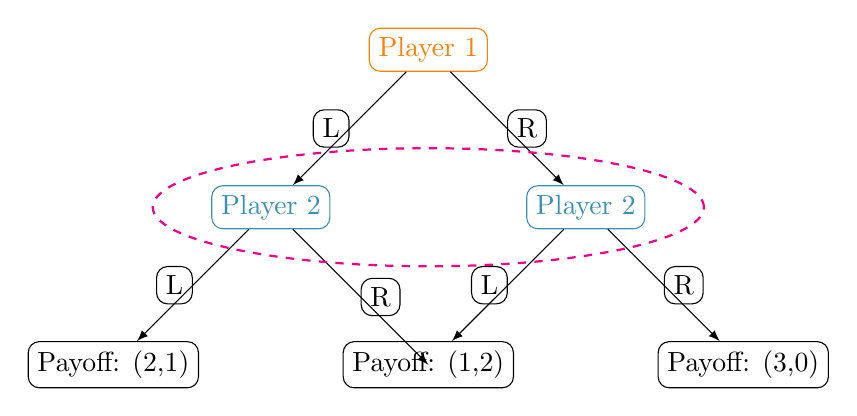
\begin{tikzpicture}[
    level distance=2cm,
    sibling distance=4cm,
    edge from parent/.style={draw,-latex},
    every node/.style={draw, rectangle, rounded corners, align=center}
  ]

% Root node (Player 1)
\node [orange]{Player 1}
    child {node[cyan!70!black] {Player 2}
        child {node {Payoff: (2,1)} edge from parent node[left] {L}}
        child {edge from parent node[right] {R}}
        edge from parent node[left] {L}
    }
    child {node[cyan!70!black] {Player 2}
        child {node {Payoff: (1,2)} edge from parent node[left] {L}}
        child {node {Payoff: (3,0)} edge from parent node[right] {R}}
        edge from parent node[right] {R}
    };

 % Add dashed circle around Player 2 Left and Player 2 Right
  \draw[dashed, thick, magenta] (0,-2) ellipse (3.5cm and .75cm);

\end{tikzpicture}
\end{center}

From the above game tree: 
\begin{enumerate}
    \item \textcolor{magenta}{\textbf{Information set:} Where Player 2's information set consists of two nodes. This is because in a simultaneous move game, we assume Player 2 does not yet know what Player 1 has selected.}
    \item \textcolor{orange}{\textbf{Player 1:} Player 1 starts at the initial node, where they make a decision L or R and Player 2 responds. Given this is a simultaneous game, its possible to reverse the players in these positions.}
    \item \textcolor{cyan!70!black}{\textbf{Player 2:} These nodes represent the decisions possible to Player 2. Note that both actions ($L, R$) are available at both nodes. As it is required the actions from each node in an information set are the same.}
\end{enumerate}


\begin{itemize}
    \item \textbf{Finite game:} A game is called finite if each player has a finite strategy set. Conversely, a game is infinite if at least one player has an infinite strategy set.
    \item \textbf{Zero sum game:} A type of game where, when one player wins, the other loses. This is a game of pure conflict.
    \item \textbf{Information set:} A subset of a player's decision nodes. The information set represents the knowledge to a player that they are standing on a node (or set of nodes). The actions available to a player within an information set must be the same, although payoffs may vary. 
    \begin{itemize}
        \item In notation: $\mathcal{H}_i$ is the collection of player $i$'s information sets, each element denoted with $H$
        \item $C(H) \subset A$, which is the set of actions available at information set, $H$ (see actions - \ref{note-act}).
    \end{itemize}
    \item \textbf{Perfect recall:} At any point in the game, a player has perfect recall when they are able to remember all previous moves, in the order taken, and therefore know where they are on the tree.
    \item \textbf{Perfect information:} Each player knows exactly what node they are on (i.e. there is a single node in the information set). A game with perfect information will have an information set of a decision node, as opposed to a game of imperfect information. 
    \item \textbf{Common knowledge:} Games have common knowledge such that all players know the structure of the game, all players know the other players are aware of the structure, and each player knows this is true of the other players' knowledge.
    \item \textbf{Strategy vs. Action:} A \textit{strategy} is a decision rule, or complete contingent plan that specifies how a player will act in every possible situation, as a best (or not a never best) response. For example, the contingent plan will contain responses to all potential moves by opposing players. While an \textit{action} is any possible available moves or decisions by a player, regardless of the strategic value. 
    \begin{itemize}
        \item A \textit{set of strategies} is defined as $n^m$ where $n$ is the number of decisions and $m$ is the number of nodes within each information set ($m$ must be the same for all nodes in an information set).
        \item $A$ is the set of all possible \textbf{actions }in a game\label{note-act}
        \item $s_i$: $\mathcal{H}_{i} \rightarrow A$ subject to $s_i(H) \in C(H)$ for all $H \in \mathcal{H}_{i}$. So $s_i$ is the functional form which represents a strategy for a player.\label{note-strategy}
        \item $s = (s_1,...s_n)$ is a profile of strategy choices for a player, where each strategy, $s$ has an induced outcome.\label{note-profile}
        \item \textbf{Example:} with a game of rock-paper-scissor: Each player has the following pure strategies:
        \[
        S_1 = S_2 = \{\text{Rock (R)}, \text{Paper (P)}, \text{Scissors (S)}\}.
        \]
        
        The payoff matrix for Player 1 is as follows:
        
        \[
        \begin{array}{|c|c|c|c|}
        \hline
        P_1 \backslash P_2 & \text{Rock (R)} & \text{Paper (P)} & \text{Scissors (S)} \\
        \hline
        \text{Rock (R)} & (0, 0) & (-1, 1) & (1, -1) \\
        \text{Paper (P)} & (1, -1) & (0, 0) & (-1, 1) \\
        \text{Scissors (S)} & (-1, 1) & (1, -1) & (0, 0) \\
        \hline
        \end{array}
        \]
        \\
        \item \textbf{Strategies:}
        \begin{itemize}
            \item Player 1 pure strategy, plays Rock: \( s_1 = \text{Rock} \).
            \item Player 2 pure strategy plays Scissors: \( s_2 = \text{Scissors} \).
            \item The outcome would be \( (s_1, s_2) = (\text{Rock}, \text{Scissors}) \), and the payoffs would be:
                \[
                u_1(\text{Rock}, \text{Scissors}) = 1, \quad u_2(\text{Rock}, \text{Scissors}) = -1.
                \]
            \item Player 1 could play a mixed strategy:
                \[
                \sigma_1 = (p_R, p_P, p_S) = \left(\frac{1}{3}, \frac{1}{3}, \frac{1}{3}\right),
                \]
            meaning Player 1 chooses Rock, Paper, and Scissors with equal probabilities.
            \item Player 2 could play a mixed strategy:
                \[
                \sigma_2 = (q_R, q_P, q_S) = \left(0.5, 0.25, 0.25\right),
                \]
            meaning Player 2 chooses Rock with 50\% probability, and Paper and Scissors with 25\% probability each.
            \item This would result in the expected payoffs: 
                \[
                    E[u_1] = \sum_{s_1 \in S_1} \sum_{s_2 \in S_2} \sigma_1(s_1) \sigma_2(s_2) u_1(s_1, s_2),
                \]
                Similarly, Player 2's expected payoff is also:
                \[
                E[u_2] = 0. \text{ due to simplification.}
                \]
        \end{itemize}
    \end{itemize}
\end{itemize}


\subsection{Representation}

\subsubsection{Normal form games}
Normal form games (NFG) are condensed versions of a game. The expression for the NFG only captures the strategy and associated payoffs. There is no additional information provided in the mathematical expression. \\

\noindent \textbf{Definition:} A normal form game is \((I, \{S_i\}_{i \in I}, \{u_i\}_{i \in I})\), where:
\begin{itemize}
    \item \(I\) is a finite set of players, \(I = \{1, 2, \ldots, n\}\).
    \item \(\{S_i\}_{i \in I}\) denotes the collection of strategy sets, where \(S_i\) denotes the set of all strategies available to player \(i\) (see \ref{note-strategy}). The strategy, again, is the complete contingency plan for a player. 
    \begin{itemize}
        \item A strategy must be \textbf{complete}, meaning the strategy will contain actions at information sets that are never reached in a game, but are potential. 
        \item A strategy will also include an action plan which may become irrelevant based on the player's own strategy (i.e. a strategy will contain actions that are not the best move, and never taken, but nonetheless are included). 
    \end{itemize}
    \item \(\{u_i\}_{i \in I}\) the von Neumann-Morgenstern utility levels. The utility represents the collection of payoff functions, where each $u_i : S_1 \times S_2 \times \cdots \times S_n \to \mathbb{R}$ assigns a real value payout to the player \(i\) based on the strategy profile.
\end{itemize}

\subsubsection{Extended form games}
Extended (or extensive) form games (EFG) are important for depicting games where the rules differ than purely static, simultaneous move games. For example, EFGs can capture dynamic games (see \ref{DG}), where the order that players move is unique, and the information available to them is not always perfect. EFGs are often depicted by game trees.\\

\noindent Formal representation of an extended form game (EFG) is: \[
\Gamma_E = \{H, A, I, \rho(\cdot), \alpha(\cdot),\mathcal{H}, H(\cdot), \iota(\cdot), p(\cdot), u \}
\]
\noindent From this formal definition, we can characterize the components: 
\begin{itemize}
    \item $\mathcal{H}$ is a finite set of nodes
        \begin{itemize}
            \item Where $H(\cdot)$ is the function that assigns the decision nodes, $x$ to an information set, $\mathcal{H}$, such that $H(x) \in \mathcal{H}$
            \item $\mathcal{H}$ is a \textit{partition} of $X$, the entirety of the set of decision nodes
            \item It is critical to recall all decision nodes assigned to the same information set must have the same set of choices (see \ref{note-choice}, so $C(x) = C(x')$ if $H(x) = H(x')$
        \end{itemize}
    \item $A$ is the finite set of actions (\ref{note-act})
    \item $I$ is the set of players
    \item $p(\cdot)$ is a function, $\mathcal{H} \rightarrow \{ \mathcal{H } \cup \emptyset$ specifying a single, immediate predecessor of each node, $x$. So, for every $x \in \mathcal{H}$ $p(x)$is non-empty, except for the case of the initial node, $x_0$
    \item \textbf{Successor}: $s(\cdot)$ is then the successor node of $x$, where $s(x) = p^{-1}(x)$. It is required that the sets of $p(x)$ and $s(x)$ are disjoint, to ensure a tree structure. 
    \item \textbf{$\alpha$}: $\alpha: X$\textbackslash$\{x_0\} \rightarrow A$ where $\alpha$ is the function of the set of actions that results in the successor nodes. The function then gives (or represents) the actions that lead any non-initial node, $x$ from its predecessor. It satisfies the property $x'. x'' \in s(x)$ and $x' \neq x'' \implies \alpha(x') \neq \alpha(x'')$.
    \item \textbf{Choices}:\label{note-choice} represented $C(x)$ are the available moves at a decision node, represented as: \[
    C(x) = \big\{a \in A: a = \alpha(x') \text{ for all } x' \in s(x)\}
    \]
    \item \textbf{$\iota(\cdot)$}: This is a function such that $\mathcal{H} \rightarrow \{0,1,... I\}$ it assigns information sets within $\mathcal{H}$ to a player, who moves at the decision nodes in the set. 
    \item \textbf{$\rho(\cdot)$}: This is a function such that $\mathcal{H}_{0} x A \rightarrow [0,1]$, which assigns probabilities to actions at information sets, where nature moves. The function satisfies 
    \[
    \rho(H, a) = 0 \text{ if } a \notin C(H) \text{ and } \sum_{a \in C(H)} \rho(H,a) = 1 \text{ for all } H \in \mathcal{H}_0
    \]
    \item \textbf{Payoff function}: $u = \{u_{1}(\cdot), u_{2}(\cdot), ... u_{I}(\cdot) \}$ is a collection of payoff functions which assign a utility representation to each player at each terminal node that can be reached. Therefore, each player has a utility, $u_i$ such that $T \rightarrow \mathbb{R}$, where $u_i$ has a Bernoulli Distribution (see \ref{berno}). 
    
\end{itemize}

\noindent For an extended form game to be operate, the following three definitions for finiteness need to hold:
\begin{enumerate}
    \item Players have a finite number of possible actions, this limits the number of potential nodes in an information set. So we rule out a game with $[a,b] \subset \mathbb{R}$ possible actions. 
    \item The game must end in a finite number of moves, implying the number of decision nodes is finite. 
    \item We also assume a finite number of players.

\noindent Nash equilibrium of an extensive form game is the same in definition, but the notion of \textit{strategy} changes. Where a strategy is now defined for \textit{every information set}. 


\end{enumerate}



\subsection{Problem types}
\begin{itemize}
    \item \textbf{Matching pennies:} The Matching Pennies game is a two-player, zero-sum game where both players simultaneously choose either Heads (H) or Tails (T). If their choices match, Player 1 wins; if they differ, Player 2 wins.

        \[
        \begin{array}{c|cc}
            & H_2 & T_2 \\
            \hline
            H_1 & (1,-1) & (-1,1) \\
            T_1 & (-1,1) & (1,-1)
        \end{array}
        \]
        
        Where, payoffs are given as \textit{(Player 1, Player 2)}.
        \begin{itemize}
            \item $(H_1, T_1)$ are Player 1's choices.
            \item $( H_2, T_2)$ are Player 2's choices.
        \end{itemize}
       
        
        This game has no pure strategy Nash equilibrium (discussed in \ref{nash}), but there exists a \textit{mixed strategy equilibrium.} where each player chooses H or T with equal probability \( (p = 0.5) \).  

    \item \textbf{Prisoner's Dilemma:}
            The Prisoner's Dilemma is a two-player, non-zero-sum game where each prisoner must decide whether to cooperate (C) or defect (D) without knowing what the other will do. The payoffs follow:
            \begin{itemize}
                \item Mutual Cooperation: Both prisoners receive a moderate sentence.
                \item Mutual Defection: Both get a severe sentence.
                \item One defects while the other cooperates: The defector goes free while the cooperator gets the harshest sentence.
            \end{itemize}        
        \[
        \begin{array}{c|cc}
            & C_2 & D_2 \\
            \hline
            C_1 & (-2,-2) & (-5,0) \\
            D_1 & (0,-5) & (-4,-4)
        \end{array}
        \]
        
        Where, payoffs are given as (Prisoner 1, Prisoner 2):
        \begin{itemize}
            \item $(C_1, D_1)$ are Player 1’s choices (Cooperate or Defect).
            \item $( C_2, D_2)$ are Player 2’s choices.  
        \end{itemize}
        
        The \textit{dominant strategy} for each player is to defect, $D$, leading to a Nash equilibrium at $(D, D)$, even though $(C, C)$ would be socially optimal.
                           
    \item \textbf{Hotelling's game}: Hotelling’s Location Model describes a competition between two firms choosing locations along a linear market (e.g., a street, a beach, or a town). Consumers are uniformly distributed across this space, and they purchase from the nearest firm. Firms strategically place themselves to capture market share, and the goal is to maximize profits, which depend on how many customers choose each firm.

    Let the two firms (Firm A and Firm B) choose their locations \( x_A \) and \( x_B \) along a unit interval \( [0,1] \). The payoffs represent the proportion of customers each firm captures:

        \[
        \begin{array}{c|ccc}
            & x_B = 0 & x_B = 0.5 & x_B = 1 \\
            \hline
            x_A = 0 & (0.5, 0.5) & (0.75, 0.25) & (1,0) \\
            x_A = 0.5 & (0.25, 0.75) & (0.5, 0.5) & (0.75, 0.25) \\
            x_A = 1 & (0,1) & (0.25, 0.75) & (0.5, 0.5)
        \end{array}
        \]

        Where payoffs (A's market share, B's market share) are given: 
        \begin{itemize}
            \item Rows represent Firm A's choice \( x_A \).
            \item Columns represent Firm B's choice \( x_B \).
        \end{itemize}
        
        In equilibrium, both firms tend to locate at the center \( x_A = x_B = 0.5 \), known as "principle of minimum differentiation", where neither firm can improve its market share by moving.
        
        If the game is sequential, one firm (Leader) moves first, and the other (Follower) responds.
        
\begin{center}
    \textbf{Sequential Hotelling’s Game: Firm A Moves First}
\end{center}

\begin{center}
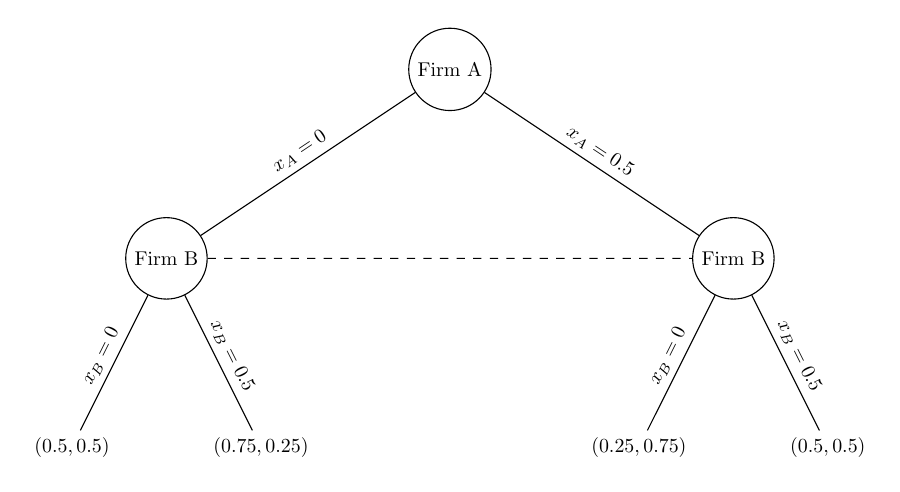
\begin{tikzpicture}[scale=1.2, transform shape, every node/.style={scale=0.6}]
    % Firm A's decision node
    \node[draw, circle] (A) at (0,0) {Firm A};
    
    % Firm B's decision nodes
    \node[draw, circle] (B1) at (-3,-2) {Firm B};
    \node[draw, circle] (B2) at (3,-2) {Firm B};
    
    % Payoff nodes
    \node (P1) at (-4,-4) {\( (0.5,0.5) \)};
    \node (P2) at (-2,-4) {\( (0.75,0.25) \)};
    \node (P3) at (2,-4) {\( (0.25,0.75) \)};
    \node (P4) at (4,-4) {\( (0.5,0.5) \)};
    
    % Connecting Firm A to Firm B
    \draw[-] (A) -- (B1) node[midway, above, sloped] {\( x_A = 0 \)};
    \draw[-] (A) -- (B2) node[midway, above, sloped] {\( x_A = 0.5 \)};
    
    % Connecting Firm B to outcomes
    \draw[-] (B1) -- (P1) node[midway, above, sloped] {\( x_B = 0 \)};
    \draw[-] (B1) -- (P2) node[midway, above, sloped] {\( x_B = 0.5 \)};
    \draw[-] (B2) -- (P3) node[midway, above, sloped] {\( x_B = 0 \)};
    \draw[-] (B2) -- (P4) node[midway, above, sloped] {\( x_B = 0.5 \)};
    
    % Dashed information set connecting Firm B's nodes
    \draw[dashed] (B1) -- (B2);
\end{tikzpicture}
\end{center}

        \begin{itemize}
            \item \textit{Simultaneous Play (Normal Form)}: The Nash equilibrium occurs when both firms locate at \( x = 0.5 \), as neither can gain an advantage by moving.
            \item \textit{Sequential Play (Extensive Form)}: The first-mover (Leader) might have an advantage by committing to a position that makes it unattractive for the second firm to differentiate too much.
        \end{itemize}

\end{itemize}

%----------------SIMULTANEOUS GAMES - SEC 2 %--------------------%
\section{Simultaneous Games}
\subsection{MWG: 7, 8, JR: 7.2, 7.3}

\subsection{Pure strategy}

A pure strategy is a deterministic strategy fro player $i$, defined on each information set. For ease, it can be helpful to think of a pure strategy as a special case of a mixed strategy, in which the probability distribution of the elements of $S_i$ is degenerate. 

A pure strategy set is represented as: \[
S_i = \{ s_{1,i}, s_{2,i},..., s_{M,i}\} \text{ for } M \text{ strategies }
\]
where the $M$ pure strategies are associated with points of a simplex, $\triangle(S_i)$, such that: \[
\triangle(S_i) = \{(\sigma_{1,i},...\sigma_{M,i}) \in \mathbb{R}^M : \sigma_{M,i} \geq 0 \text{ for all } m = 1,...M \text{ and } \sum^{M}_{m=1} \sigma_{mi} = 1 \}
\]


\subsection{Mixed strategy}
A mixed strategy for player \(i\) is a probability distribution \(\sigma_i \in \Delta(S_i)\), where \(\Delta(S_i)\) represents the set of all probability distributions over the pure strategies \(S_i\). For a finite pure strategy set \(S_i\), a mixed strategy \(\sigma_i : S_i \to [0, 1]\) assigns a probability \(\sigma_i(s_i)\) to each pure strategy \(s_i \in S_i\), such that:
\[
\sum_{s_i \in S_i} \sigma_i(s_i) = 1 \quad \text{and} \quad \sigma_i(s_i) \geq 0 \quad \forall s_i \in S_i.
\]

\noindent \textbf{A mixed strategy represents a probabilistic choice}, capturing the expected behavior of a player. Unlike pure strategies, which yield deterministic payoffs, the payoff from a mixed strategy is not deterministic; it reflects the expected value over the possible outcomes. A mixed strategy may be used if you receive some private signal, $\Theta$ with a $N(0,1)$ distribution, and then you will form a plan of action based on the realization of the signal. The game, with a mixed strategy, is still represented as: \[
\Gamma_{N} = [I, \{\triangle(S_i)\}, \{u_i(\cdot)\}]
\]

\noindent The expected payoff of player \(i\) using a mixed strategy \(\sigma_i\) against a pure strategy profile \(s_{-i}\) of the other players is given by:
\[
u_i(\sigma_i, s_{-i}) = \mathbb{E}_{s_i \sim \sigma_i}[u_i(s_i, s_{-i})] = \sum_{s_i \in S_i} \sigma_i(s_i) u_i(s_i, s_{-i}).
\]

\noindent Expected payoff of player \(i\) when all players are using mixed strategies \(\sigma = (\sigma_i, \sigma_{-i})\) is:
\[
u_i(\sigma) = \sum_{s_i \in S_i} \sum_{s_{-i} \in S_{-i}} [\sigma_i(s_i) \sigma_{-i}(s_{-i})] u_i(s_i, s_{-i}).
\]

\noindent \textbf{Relationship between a mixed and pure strategy:} For player \(i\), a mixed strategy \(\sigma_i \in \Delta(S_i)\) strictly dominates (\textit{see \ref{dom}}) a pure strategy \(s'_i \in S_i\) if, for all \(s_{-i} \in S_{-i}\),
\[
u_i(\sigma_i, s_{-i}) > u_i(s'_i, s_{-i}).
\]
\begin{itemize}
    \item The set of pure strategies is a \textbf{proper subset} of the set of mixed strategies: $S_i \subset \Delta(S_i)$.
    \item Player $i$'s set of possible mixed strategies are represented as a set of points in a simplex (where a simplex is the smallest convex set that contains a given set of points).
    \item A mixed strategy uses \textbf{randomization}, such that the choices, in each information set, are randomized, resulting in a distribution of probabilities across the terminal nodes of the game and an random, induced outcome of the game. 
\end{itemize}


\subsection{Rationality}\label{rationality}
\textbf{Definition:} Player \( i \) is said to be rational when playing strategy \( s_i \in S_i \) with belief \( \mu_i \in \Delta(S_{-i}) \), if and only if \( s_i \) is a best response to some belief \( \mu_i \). That is, a player \( i \) is rational if, given their belief \( \mu_i \) about other players' strategies, they choose a strategy \( s_i \) that maximizes their expected payoff. Formally, for every \( s_i' \in S_i \) with \( s_i' \neq s_i \):
\[
\mathbb{E}_{s_{-i} \sim \mu_i} \big[ u_i(s_i, s_{-i}) \big] \geq \mathbb{E}_{s_{-i} \sim \mu_i} \big[ u_i(s_i', s_{-i}) \big],
\]

\noindent \textbf{What is rationality in a game?}
\begin{itemize}
    \item The \textbf{rules of the game} imply rationality when we assume all players are rational, and believe that the other players are also rational, and the players know the others are rational, and so on. 
    \item \textbf{A player is rational} if he never plays a strictly dominated strategy.
    \item In finite games, \textbf{the set of rationalizable strategies} is the set of strategies that survive iterated strategic dominance with pure strategies. That is, rationalizable strategies cannot be never-best-responses (NBRs). 
\end{itemize} 


\noindent Other definitions which define rationalizability at different stategies of the game:
\begin{itemize}
    \item A \textit{1-rationalizable strategy} for player \( i \) is an element of \( S_i \) that is a best response to some belief \( \mu_i \) over other player strategies.
    \item A \textit{k-rationalizable strategy} for player \( i \) is an element of \( S_i \) that is a best response to some belief \( \mu_i \) over \( k-1 \) rationalizable strategies of other players.
    \item A \textit{rationalizable strategy} for player \( i \) is an element of \( S_i \) that is \( k \)-rationalizable for every \( k \).
\end{itemize} \\

In words, a \textit{1-rationalizable strategy} is one that can be a best response to any belief about what others might play, assuming they are rational. A \textit{k-rationalizable strategy} is optimal when players expect others to choose from their \( (k-1) \)-rationalizable strategies. Ultimately, a \textit{rationalizable strategy} is one that remains optimal no matter how many rounds of reasoning are applied, i.e., it is consistently a best response to rational expectations of others' rational behavior. \\ 

\noindent \textbf{Sequential rationality:} \\
\\
\textbf{Definition - System of Beliefs:} \\
A system of beliefs $\mu$ in an extensive form game $\Gamma_E$ is a specification of a probability $\mu(x) \in [0,1]$ for each decision node $x$ in $\Gamma_E$ such that:
\[
\sum_{x\in H} \mu(x) = 1
\]
for all information sets $H$.
\\
\\
\textbf{Definition - Sequential Rationality of Strategies:} \\
Consider an extensive form game $\Gamma_E$, an information set $H$, the player who moves there, $i$, and $i$'s system of beliefs $\mu$. A strategy profile $\sigma = (\sigma_1, ..., \sigma_I)$ in $\Gamma_E$ is sequentially rational at $H$ given $\mu$ if:
\[
E [u_i | H, \mu, \sigma_i , \sigma_{-i} ] \geq E [u_i | H, \mu, \tilde{\sigma}_i , \sigma_{-i} ]
\]
for all $\tilde{\sigma}_i \in \Delta(S_i)$.



\subsubsection{Iterated dominance}\label{ISD}

To find \textbf{rationalizable strategies}, we required that the remaining strategies (after iterative removal of the NBRs) were the best responses to some conjectures, not to actual play. We delete \textit{strictly dominated strategies} iteratively until nothing else can be deleted. With each iteration, additional strategies might become dominated (the case of weakly dominated strategies will be dealt with later). \\
\\
\noindent \textbf{A player must now know} not only that her rivals are rational but also that they know that she is, and so on. This is why IDDS relies on the concept of rationality. After iterated deletion of dominated strategies (IDDS), the set of rationalizable strategies can be no larger than the set of strategies surviving IDDS. 
\\
\\
\noindent \textbf{Steps to eliminating strictly dominated strategies: }
\begin{enumerate}
    \item Consider only the set of pure strategies
    \item Eliminate strictly dominated strategies 
    \item Consider which mixed strategies are undominated
    \begin{itemize}
        \item Eliminate mixed strategies which have a pure, dominated strategy within the mixed strategy
        \item Look at, and compare, expected payoffs (as some randomization may create new, dominant strategies)
    \end{itemize}
\end{enumerate}

\begin{table}[h]
    \centering
    \renewcommand{\arraystretch}{1.3}
    \begin{tabular}{|p{7cm}|p{7cm}|}
        \hline
        \textbf{Benefits of IDDS} & \textbf{Limitations of IDDS} \\
        \hline
        The order of elimination is irrelevant. & Won’t always reach a solution. \\
        There is no need to know the other player’s action. & We must assume common knowledge of rationality and of the game. \\
        It all comes from rationality. & It often leads to inefficient outcomes. \\
        \hline
    \end{tabular}
    \caption{Comparison of Benefits and Limitations of Strict Iterative Elimination}
    \label{table:elim_benefits_vs_limitations}
\end{table}

\noindent \textbf{Propositions:}
\begin{enumerate}
    \item The set of surviving strategy profiles is invariant to the order of elimination of strictly dominated strategies.
    \item If, at the end of this process, only a single profile remains, then it is called the iterated deletion of strictly dominated strategies (IDDS) solution of that game, the game is said to be dominance solvable.
\end{enumerate}

\subsubsection{Best response}
If a strategy is strictly dominant (see \ref{dom}), then it is also a best response, where the player's payoff is maximized, regardless of the other player's response. \\
\\
\noindent \textbf{Definition - best response:} In game \(\Gamma_N = [I, \{\Delta(S_i)\}, \{u_i(\cdot)\}]\), strategy \(\sigma_i\) is a \textit{best response} for player \(i\) to his rivals' strategies \(\sigma_{-i}\) if
\[
u_i(\sigma_i, \sigma_{-i}) \geq u_i(\sigma_i', \sigma_{-i})
\]
for all \(\sigma_i' \in \Delta(S_i)\).
\\
\noindent Strategy \(\sigma_i\) is a best response to \(\sigma_{-i}\) if it is an optimal choice when player \(i\) \textit{conjectures} that his opponents will play \(\sigma_{-i}\).
\\
\\
\noindent \textbf{Never best response:} Strategy $sigma_i$ is a never best response if there is no $\sigma_{-i}$ for which $sigma_i$ is a best response. This implies that $sigma_i$ cannot be justified in rational play. 
\begin{itemize}
    \item Any strategy that is \textit{strictly dominated} is never a best response.
    \item Never best responses contain the set of strictly dominated strategies. But, recall that strictly dominated strategies is a \textit{smaller} set than the set of NBRs. 
    \item The order of removal of strategies that are NBR does not affect the set of surviving strategies. 
\end{itemize}


\subsection{Dominance}\label{dom}

\noindent Dominance provides a prediction for what moves will be played, based on the most obvious way to compare a player's strategy (ignore randomization over pure strategies at this point). So, dominance, in this case, shows a player's payoff is maximized (in the case of strict dominance) if player's payoff is uniquely highest, regardless of the opponent's move. \\ 
\\
Dominance is a key subject for eliminating alternatives when evaluating a game. For example, we use \textbf{iterated removal} \textit{(discussed in depth in \ref{ISD})} to eliminate \textit{dominated strategies}, resulting in a unique set of strategies. \\

\subsubsection{Strictly, weakly dominant}
Any strategy where, regardless of what the opposing player does, there is a best move to take. This means that for all of the opposing player(s)' moves, there exists a strategy that is strictly better, regardless of these strategies. Strictly dominant strategies rarely exist, but we know that when they do, they uniquely maximize player $i$'s payoff, regardless of the rivals' moves. \\
\\
\noindent \textbf{Definition:} A strategy $s_i \in S_i$ is \textbf{strictly dominant} for player $i$ in game $\Gamma_N = [I, \{S_i\}, \{u_{i}(\cdot)\}]$ if for all $s_{i}' \neq s_i$ we have: \[
u_{i}(s_{i}, s_{-i}) > u_{i}(s_{i}', s_{-i})
\] 
for all $s_{i}' \in S_{-i}$ \\

\noindent In a case with \textbf{mixed strategies}, we check whether any of player $i$'s mixed strategies does better than his pure strategy, $s_i$, against every possible pure strategy profile by player $j$. Player $i$'s pure strategy $s_i \in S_i$ is strictly dominant in a game if and only if, for all $\sigma_{i}' \in \triangle(S_i)$ such that \[
u_{i}(\sigma_{i}', s_{-i}) > u_{i}(s_{i}, s_{-i})
\]
for all $s_{-i} \in S_{-i}$
 
\subsubsection{Strictly, weakly dominated}

\noindent \textbf{Definition:} A strategy $s_i \in S_i$ is \textbf{strictly dominated }for player $i$ in game $\Gamma_N = [I, \{S_i\}, \{u_{i}(\cdot)\}]$ if there exists another strategy $s_{i}' \in S_i$ such that for all $s_{-i} \in S_{-i}$: \[
u_{i}(s_{i}', s_{-i}) > u_{i}(s_{i}, s_{-i})
\] 
where strategy $s_{i}'$ dominates strategy $s_i$



\subsection{Nash Equilibrium}\label{nash}
Up to now, we have only imposed the assumption of \textit{common rationality}. But rationality leaves us with too many possible strategies. To refine the set of possible outcomes and identify a solution to the game, additional assumptions are required. The concept of Nash Equilibrium introduces two critical assumptions: \textbf{mutual best responses} and \textbf{mutual correct expectations}. Together,
these conditions create a stable outcome where no player has an incentive to deviate unilaterally.
\begin{itemize}
    \item Mutual best responses ensure that each player’s chosen strategy is optimal given the strategies actually played by others.
    \item Mutual correct expectations mean that players’ beliefs about each other’s strategies align perfectly.
\end{itemize} 
Since a nash equilibrium is a situation where each player's chosen strategy is the best possible response to the strategies chosen by others, no player has an incentive to unilaterally change their strategy, as doing so would not improve their payoff. This ensures that the outcome is stable.
\\

\textbf{Formal definition:} A strategy profile \((s_1, \ldots, s_n)\) is a pure strategy Nash equilibrium (NE) if for all players \(i\), and for all \(s_i' \in S_i\) with \(s_i' \neq s_i\),
\[
    u_i(s_i, s_{-i}) \geq u_i(s_i', s_{-i}).
\]
 
\subsection{Existence of Nash Equilibrium}

The following theorem is a \textbf{sufficient condition} for the existence of a nash equilibrium. \\

\textbf{Theorem:} Let \(S_1, \ldots, S_n\) be compact and convex subsets of \(\mathbb{R}^K\), and let \(u_i\) be a continuous and quasiconcave function in \(s_i\) for each player \(i\). Under these conditions, a pure strategy Nash equilibrium exists.
\\
\textbf{Proof:}

For each player \(i\), define their best response correspondence as:
\[
    BR_i(s_{-i}) = \arg\max_{s_i \in S_i} u_i(s_i, s_{-i}).
\]

The combined best response correspondence is:
\[
    BR(s) = \big(BR_1(s_{-1}), \ldots, BR_n(s_{-n})\big).
\]

Then, a strategy profile \(s = (s_1, \ldots, s_n)\) is a Nash equilibrium if \(s \in BR(s)\). Use Kakutani’s Fixed Point Theorem to show that such a strategy profile exists. To apply Kakutani’s theorem (see \ref{kak}), verify the following required properties of \(BR_i(s_{-i})\):
\begin{itemize}
    \item \textbf{Non-Empty Valued:} Since \(u_i\) is continuous in \(s_i\) and \(S_i\) is compact, the maximum of \(u_i(s_i, s_{-i})\) over \(s_i \in S_i\) is attained (by the Weierstrass Theorem, see \ref{weiss}). Therefore, \(BR_i(s_{-i})\) is non-empty for all \(s_{-i}\).
    
    \item \textbf{Upper Hemicontinuity:} Suppose, toward contradiction, that \(BR_{i}\) is not upper hemicontinuous at \(s^{*}_{-i}\). Then there exist sequences \(s^t_{-i} \to s^*_{-i}\) and \(s^t_{i} \in BR_i(s^{t}_{-i})\) such that $(s^{t}_{i} \to s_{i}' \notin BR_{i}(s_{-i}^{*})$. \\ 

    Since \(s_{i}' \notin BR_{i}(s^{*}_{-i})\), there exists \(s^{*}_{i} \in S_{i}\) such that:
    \[
        u_i(s^*_{i}, s^*_{-i}) > u_i(s'_{i}, s^*_{-i}).
    \]

    By continuity of \(u_i\):
    \[
        u_i(s^t_{i}, s^t_{-i}) \to u_i(s'_i, s^*_{-i}), \quad u_i(s^*_{i}, s^t_{-i}) \to u_i(s^*_{i}, s^*_{-i}).
    \]

    Therefore, for sufficiently large \(t\):
    \[
        u_i(s^*_{i}, s^t_{-i}) > u_i(s^t_{i}, s^t_{-i}),
    \]
    which implies \(s^t_i \notin BR_i(s^t_{-i})\), a contradiction.
    
    \item \textbf{Convex-Valued:} Suppose \(s'_i, s''_i \in BR_i(s_{-i})\), then:
    \[
        u_i(s'_{i}, s_{-i}) = u_i(s''_{i}, s_{-i}) = g^*.
    \]
    For any \(\lambda \in [0, 1]\), the quasiconcavity of \(u_i\) implies:
    \[
        u_i(\lambda s'_i + (1 - \lambda)s''_i, s_{-i}) \geq g^*.
    \]
    Since \(g^*\) is the maximum as \(s'_i, s''_i \in BR_i(s_{-i})\), equality holds:
    \[
        u_i(\lambda s'_i + (1 - \lambda)s''_i, s_{-i}) = g^.
    \]
    Therefore, \(\lambda s'_i + (1 - \lambda)s''_i \in BR_i(s_{-i})\), proving that \(BR_i(s_{-i})\) is convex.
\end{itemize}

Having verified all the conditions of Kakutani’s Fixed Point Theorem, there exists \(s^* \in S\) such that:
\[
    s^* \in BR(s^*).
\]

Such \(s^*\) is the pure strategy Nash equilibrium. \\ 

\noindent \textbf{Computing Randomized Nash Equilibria}: 
We are given some game, including a given set of players \( N \) and, for each \( i \in N \), a given set of feasible actions \( C_i \) for player \( i \) and a given payoff function \( u_i: C_1 \times \dots \times C_n \to \mathbb{R} \) for player \( i \).


\noindent The \textbf{support} of a randomized equilibrium is, for each player, the set of actions that have positive probability of being chosen in this equilibrium. To find a Nash equilibrium, we can apply the following 5-step method:

\begin{enumerate}
    \item \textbf{Guess a support for all players.} That is, for each player \( i \), let \( S_i \) be a subset of \( i \)'s actions \( C_i \), and let us guess that \( S_i \) is the set of actions that player \( i \) will use with positive probability.

    \item \textbf{Consider the smaller game where the action set for each player is reduced to \( S_i \).} Try to find an equilibrium where all of these actions get positive probability.
    
    To do this, we need to solve a system of equations for some unknown quantities.

    \begin{itemize}
        \item \textbf{Unknowns:} For each player \( i \in N \) and each action \( s_i \) in \( i \)'s support \( S_i \), let \( \sigma_i(s_i) \) denote \( i \)'s probability of choosing \( s_i \), and let \( w_i \) denote player \( i \)'s expected payoff in the equilibrium. (\(\sigma_i(a_i) = 0\) if \( a_i \notin S_i \)).
        
        \item \textbf{Equations:} For each player \( i \), the sum of these probabilities \( \sigma_i(s_i) \) must equal 1.
        
        \item For each player \( i \) and each action \( s_i \in S_i \), player \( i \)'s expected payoff when choosing \( s_i \) while all other players randomize independently according to their \( \sigma_j \) probabilities must equal \( w_i \).

        Let \( u_i(\sigma_i, [a_i]) = \mathbb{E}[u_i(a_i | \sigma_{-i})] \) denote player \( i \)'s expected payoff when they choose action \( a_i \) and all other players are expected to randomize independently according to their \( \sigma_j \) probabilities.

        Then the equations can be written as:
        \[
        \sum_{s_i \in S_i} \sigma_i(s_i) = 1, \quad \forall i \in N
        \]
        \[
        u_i(\sigma_i, [s_i]) = w_i, \quad \forall i \in N, \forall s_i \in S_i.
        \]
    \end{itemize}

    \item \textbf{Check if the equations in step 2 have a solution.} If no solution exists, then we guessed the wrong support and must return to step 1 and guess a new support.

    \item \textbf{Verify that all probabilities are nonnegative.} If any probability is negative, then we must return to step 1 and guess a new support.

    If we have a solution that satisfies all these nonnegativity conditions, then it is a randomized equilibrium of the reduced game where each player can only choose actions in \( S_i \).

    \item \textbf{Check if the solution is an equilibrium of the original game.} A solution from step (2) that satisfies the condition in (4) is still not necessarily an equilibrium of the original game.

    For each player \( i \) and for each action \( a_i \in C_i \setminus S_i \), we must check whether choosing \( a_i \) would yield a higher payoff than \( w_i \). That is:
    \[
    u_i(\sigma_i, [s_i]) = w_i, \quad \forall s_i \in S_i.
    \]

    If, for any action \( a_i \notin S_i \), we have \( u_i(\sigma_i, [a_i]) > w_i \), then we must return to step 1 and guess a new support.

\end{enumerate}

In a finite game, there are only a finite number of possible supports to consider. Thus, an equilibrium \( \sigma = (\sigma_i(a_i))_{a_i \in C_i, i \in N} \) with payoffs \( w = (w_i)_{i \in N} \) must satisfy:

\[
\sum_{a_i \in C_i} \sigma_i(a_i) = 1, \quad \forall i \in N;
\]
\[
\sigma_i(a_i) \geq 0, \quad u_i(\sigma_{-i}, [a_i]) \leq w_i, \quad \text{with at least one equality (complementary slackness) for all } a_i \in C_i, \forall i \in N.
\]

The support for each player \( i \) is the set of actions \( s_i \in C_i \) for which \( \sigma_i(s_i) > 0 \), so that \( u_i(\sigma_{-i}, [s_i]) = w_i \).


\subsection{Problem types}



%------------------DYNAMIC GAMES - SEC 4 %---------------------%
\section{Dynamic games}\label{DG}

\subsection{Backward induction}

\subsection{Sub-game perfect Nash Equilibrium}

\subsection{Problem types}


%------------------INCOMPLETE INFO - SEC 5 %---------------------%
\section{Incomplete information}\label{II}

\subsection{Bayesian games}\label{bayes}

\subsection{Bayesian nash equilibrium concepts}\label{WPBNE}

\textbf{Bayesian Nash Equilibrium}: a strategy profile \(\{s_i(\theta_i)\}\) such that each player maximizes their expected utility given their beliefs about the types of other players:
\[
E[u_i(s_i(\theta_i), s_{-i}(\theta_{-i}) | \theta_i] \geq E[u_i(s_i', s_{-i}(\theta_{-i}) | \theta_i], \quad \forall s_i' \in S_i, \quad \forall \theta_i \in \Theta_i.
\]


\textbf{Definition: Weak Perfect Bayesian Equilibrium (WPBE)} \\
A profile of strategies and system of beliefs $(\sigma, \mu)$ is a weak perfect Bayesian equilibrium (WPBE) in an extensive form game $\Gamma_E$ if:
\begin{itemize}
    \item[(i)] The strategy profile $\sigma$ is sequentially rational given belief system $\mu$.
    \item[(ii)] The system of beliefs $\mu$ is derived from strategy profile $\sigma$ through Bayes’ rule whenever possible:
    \[
    \mu(x) = \frac{\Pr [x | \sigma]}{\Pr [H | \sigma]}, \quad \forall x \in H.
    \]
\end{itemize}
\\
\\
\textbf{Definition: Sequential Equilibrium} \\
A strategy profile and system of beliefs $(\sigma, \mu)$ is a sequential equilibrium of an extensive form game $\Gamma_E$ if:
\begin{enumerate}
    \item The strategy profile $\sigma$ is sequentially rational given belief system $\mu$.
    \item There exist:
    \begin{itemize}
        \item A sequence of completely mixed strategies converging to $\sigma$, $\{\sigma_k\}_{k=1}^{\infty} \to \sigma$.
        \item A sequence of belief systems converging to $\mu$, $\{\mu_k\}_{k=1}^{\infty} \to \mu$.
        \item Each belief system $\mu_k$ is derived from strategy profile $\sigma_k$ using Bayes’ rule.
    \end{itemize}
\end{enumerate} 
\\
\\
\textbf{Proposition: Relationship between WPBE and Nash Equilibrium} $\Rightarrow$ A strategy profile $\sigma$ is a Nash equilibrium of an extensive form game $\Gamma_E$ if and only if there exists a system of beliefs $\mu$ such that:
\begin{enumerate}
    \item Strategy profile $\sigma$ is sequentially rational given $\mu$ at all info sets $H$ such that $\Pr [H | \sigma] > 0$.
    \item The system of beliefs $\mu$ is derived from $\sigma$ through Bayes’ rule whenever possible.
\end{enumerate}
Every WPBE is a Nash equilibrium, but not all Nash equilibria are WPBE.


\subsection{Asymmetric information}

\subsubsection{Adverse selection (in the labor market)}

\subsubsection{Signalling (in the labor market)}

\textbf{Lemma: Separating Equilibria in Signaling Games}: In any \textbf{separating Perfect Bayesian Equilibrium (PBE)}, the equilibrium wages satisfy:
\[
w^*(e^*(\theta_H)) = \theta_H, \quad w^*(e^*(\theta_L)) = \theta_L.
\]
That is, each worker type receives a wage equal to her productivity level.




%------------------OLIGOPOLIES- SEC 6 %---------------------%
\section{Static oligopoly models}\label{SO}

\subsection{Bertrand Competition}

\textbf{Propositions:}
\begin{itemize}
    \item \textbf{Subgame Perfect Nash Equilibrium in Bertrand Duopoly}: The strategies described for price-setting in Bertrand duopoly constitute a \textbf{subgame perfect Nash equilibrium (SPNE)} if and only if $\delta \geq 1/2$.
    
    \item \textbf{SPNE in Infinitely Repeated Bertrand Duopoly}: In an infinitely repeated \textbf{Bertrand duopoly game}, when $\delta \geq 1/2$, repeated choice of any price $p \in [c, p_m]$ can be supported as an \textbf{SPNE outcome path} using Nash reversion strategies.

\end{itemize}




\subsection{Cornout Competition}

\subsection{Repeated Games}

\textbf{Definition: Nash Reversion Strategy in Repeated Games} \\
A strategy profile $s = (s_1, ..., s_I)$ in an infinitely repeated game is one of \textbf{Nash reversion} if each player’s strategy calls for playing some outcome path $Q$ until someone defects and playing the stage game \textbf{Nash equilibrium} $q^* = (q^*_1, ..., q^*_I)$ thereafter.
\\

\textbf{Propositions:}
\begin{itemize}
    \item \textbf{Folk Theorem for Repeated Games}: In an infinitely repeated game, any feasible discounted payoffs that give each player, on a per-period basis, more than the lowest payoff that they could guarantee in a \textbf{single-play simultaneous-move component game}, can be sustained as the payoffs of an \textbf{SPNE} if players discount the future sufficiently.

    \item \textbf{Sustaining Cooperation in Repeated Games}: If there is potential for joint improvement in payoffs near the stage game \textbf{Nash equilibrium}, then for sufficiently high $\delta$, there exists a \textbf{subgame perfect equilibrium (SPNE)} where payoffs exceed those in the static \textbf{Nash equilibrium}. 
    
    \item \textbf{Credible Punishment in Repeated Games}: If each player’s stage game Nash equilibrium payoff strictly exceeds their minimax payoff, then there exists an SPNE with more severe punishments than Nash reversion 
\end{itemize}
\\

\textbf{Lemma 1: Nash Reversion Strategies and SPNE}: A Nash reversion strategy profile that calls for playing outcome path $Q = \{q_{1t} , ..., q_{It}\}_{t=1}^{\infty}$ prior to any deviation is an \textbf{SPNE} if and only if:
\[
\hat{\pi}_i(q_{-it}) + \frac{d}{1 - d} \pi_i(q^*) \leq v_i(Q, t), \quad \forall t, i
\]
where $\hat{\pi}_i(\cdot)$ denotes player $i$’s payoff from deviating and $q^*$ is the stage game Nash equilibrium.



%------------------APPENDIX %---------------------%

\section{Appendix}

\subsection{Mathematical forms of games}

\subsection{Example game trees}
Prisoner's dilemma 
Foggy oil tanker 
Hotelling's problem 
Matching pennies 

\subsection{Fundamental welfare theorems}
\begin{enumerate}
    \item In a perfectly competitive market, any equilibrium allocation of resources is pareto efficient (i.e. no individual can be made better off without making someone else worse off).
    \item Any pareto efficient allocation can be achieved by having a competitive market equilibrium, provided that the appropriate redistribution of initial endowments is implemented (i.e. markets make efficient outcomes where the initial distribution of resources can bve adjusted). 
\end{enumerate}


\subsection{Other theorems}
\subsubsection{Weierstrass Theorem}\label{weiss}
\textbf{Theorem:} Let \(f: S \to \mathbb{R}\) be a continuous real-valued function, where \(S \subseteq \mathbb{R}^n\) is a non-empty, compact set. Then \(f\) attains its maximum and minimum on \(S\). That is, there exist \(x^, x_ \in S\) such that:
\[
f(x_) \leq f(x) \leq f(x^) \quad \text{for all } x \in S.
\]

\textbf{Definition:} Any continuous function defined on a non-empty, compact set has both a maximum and a minimum value. This theorem is necessary for proving the existence of nash equilibria under standard conditions, by ensuring that the utility function has a maximum. 

\subsubsection{Core mathematical properties:}

\begin{itemize}

    \item \textbf{Convex Set}:
    A set \( X \subseteq \mathbb{R}^n \) is \textbf{convex} if, for any \( x, y \in X \) and \( \alpha \in [0, 1] \), the combination
    \[
    \alpha x + (1 - \alpha) y \in X.
    \]

    \item \textbf{Quasiconcave Function}:
    A function \( f : \mathbb{R}^n \to \mathbb{R} \) is \textbf{quasiconcave} if, for any \( x, y \in X \) and \( \alpha \in [0, 1] \),
    \[
    f(\alpha x + (1 - \alpha) y) \geq \min\{f(x), f(y)\}.
    \]

    \item \textbf{Correspondence}:
    A \textbf{correspondence} \( r : X \rightrightarrows Y \) is a set-valued function from \( X \) to subsets of \( Y \).
    \begin{itemize}
        \item It is \textbf{convex valued} if, for all \( x \in X \), \( r(x) \) is convex.
        \item It is \textbf{upper hemicontinuous} if, for every sequence \( x^t \to x \) and \( y^t \to y \) with \( y^t \in r(x^t) \) for all \( t \), we have \( y \in r(x) \).
        
        \textit{(Intuition: A correspondence \( r : X \rightrightarrows Y \) is upper hemicontinuous if the set \( r(x) \) "shrinks nicely" as \( x \) approaches a limit. Specifically, if \( x^t \to x \) and \( y^t \in r(x^t) \) with \( y^t \to y \), then \( y \in r(x) \). This ensures that \( r(x) \) does not include any "new" elements not approached by \( r(x^t) \).)}
    \end{itemize}

    \item \textbf{Compact Set}:
    A set \( K \subseteq \mathbb{R}^n \) is \textbf{compact} if it is both:
    \begin{itemize}
        \item \textbf{Closed}: \( K \) contains all its boundary points.
        \item \textbf{Bounded}: \( K \) fits within some finite region of \( \mathbb{R}^n \).
    \end{itemize}
    In other words, \( K \) is compact if it is a closed and bounded subset of \( \mathbb{R}^n \).

    \item \textbf{Bernoulli distribution:}\label{berno}
        A discrete random variable \( X \) follows a Bernoulli distribution with parameter \( p \), where \( 0 \leq p \leq 1 \), if it takes values in \( \{0,1\} \) with probability mass function (PMF) given by:
        
        \[
        P(X = x) =
        \begin{cases}
            p, & \text{if } x = 1, \\
            1 - p, & \text{if } x = 0.
        \end{cases}
        \]
        
        This is denoted as:
        
        \[
        X \sim \text{Bern}(p).
        \]
        
        The expected value and variance of \( X \) are:
        
        \[
        E[X] = p, \quad \text{Var}(X) = p(1 - p).
        \]
\end{itemize}

\subsubsection{Kakutani's Fixed Point Theorem}\label{kak}

\textbf{Theorem 2:} Let \( X \neq \emptyset \) be a compact and convex subset of \( \mathbb{R}^K \), and let \( r : X \rightrightarrows X \) be a correspondence such that:
\begin{itemize}
    \item \( r \) is non-empty valued,
    \item \( r \) is convex valued,
    \item \( r \) is upper hemicontinuous.
\end{itemize}
Then, there exists \( x \in X \) such that \( x \in r(x) \), i.e., \( r \) has a fixed point.




% Table begins here
\renewcommand{\arraystretch}{1.5} % Increase row height for better readability
\begin{table}[h!]
\centering
\begin{tabular}{@{}m{0.35\textwidth} m{0.3\textwidth} m{0.3\textwidth}@{}}
\toprule
\textbf{Mathematical Formula} & \textbf{Description of Items} & \textbf{Description of the Game} \\
\midrule
\textbf{Normal Form (Mixed Game)}\\
$\Gamma_N = \big[I, \{\Delta(S_i)\}, \{u_i(\cdot)\}\big]$ & \begin{itemize}
  \item $I$: Set of players
  \item $\Delta(S_i)$: Set of mixed strategies for player $i$, where $S_i$ is the set of pure strategies
  \item $u_i$: Utility function of player $i$
\end{itemize} & Describes a game where players choose mixed strategies and payoffs are determined based on mixed strategies in normal form. \\
\midrule
\textbf{Normal Form (Pure Game)}\\
$\Gamma_N = \big[I, \{S_i\}, \{u_i(\cdot)\}\big]$ & \begin{itemize}
  \item $I$: Set of players
  \item $S_i$: Set of pure strategies for player $i$
  \item $u_i$: Utility function of player $i$
\end{itemize} & Describes a game where players choose pure strategies, and payoffs are determined based on these strategies in normal form. \\
\midrule
\textbf{Extensive Form (Mixed Game)}\\
$\Gamma_E = \big[I, T, P, \{\Delta(S_i)\}, \{u_i(\cdot)\}\big]$ & \begin{itemize}
  \item $T$: Set of decision nodes
  \item $P$: Player assignment function for decision nodes
  \item $\Delta(S_i)$: Set of mixed strategies
  \item $u_i$: Utility function of player $i$
\end{itemize} & Describes a game represented as a tree, where players make decisions at each node, and mixed strategies determine probabilities of actions. \\
\midrule
\textbf{Extensive Form (Pure Game)}\\ % I MAY NEED TO ADD TO THIS A BIT -- SEE NOTES FROM CLASS 
$\Gamma_E = \big[I, T, P, \{S_i\}, \{u_i(\cdot)\}\big]$ & \begin{itemize}
  \item $T$: Set of decision nodes
  \item $P$: Player assignment function for decision nodes
  \item $S_i$: Set of pure strategies
  \item $u_i$: Utility function of player $i$
\end{itemize} & Describes a game represented as a tree, where players make decisions at each node, and strategies are pure. \\
\bottomrule
\end{tabular}
\caption{Comparison of Mixed and Pure Games in EFG and NFG}
\label{tab:games_table}
\end{table}


\begin{table}[htbp]
\centering
\small
\renewcommand{\arraystretch}{1.5}
\begin{tabular}{|p{3.5cm}|p{2.1cm}|p{4.1cm}|p{5.7cm}|}
\hline
\textbf{Concept} & \textbf{Type} & \textbf{Game Type} & \textbf{Short Description} \\ \hline
\textbf{Rationality} & Condition & Perfect, Imperfect, Adverse Selection, Signaling, Repeated & Players choose strategies maximizing expected payoffs given beliefs. \\ \hline
\textbf{Nash Equilibrium (NE)} & Equilibrium Concept & Perfect, Imperfect, Adverse Selection, Signaling, Repeated & No player can gain by unilaterally deviating from equilibrium strategies. \\ \hline
\textbf{Bayesian Nash Equilibrium (BNE)} & Equilibrium Concept & Imperfect info, Adverse Selection, Signaling & NE for incomplete information; strategies maximize expected payoffs given beliefs about others' types. \\ \hline
\textbf{Subgame Perfect Nash Equilibrium (SPNE)} & Equilibrium Refinement & Perfect info (clearly defined subgames), Repeated & NE refinement requiring equilibrium within every subgame (no non-credible threats). In repeated games, credible equilibrium strategies specifying optimal actions after every possible history, often using punishment. \\ \hline
\textbf{Weak Perfect Bayesian Equilibrium (Weak PBE)} & Equilibrium Refinement & Imperfect info, Signaling, Adverse Selection & Equilibrium requiring sequential rationality and weak consistency of beliefs (Bayesian updating where possible). \\ \hline
\textbf{Nash Reversion Strategies} & Strategy/ Punishment Method & Repeated Games & Punishment reverting permanently to stage-game NE after deviation; sustains cooperation. \\ \hline
\textbf{Sequential Rationality} & Condition & Perfect, Imperfect, Signaling, Adverse Selection, Repeated & Requires optimal actions at every decision point given beliefs. \\ \hline
\textbf{Backward Induction} & Method & Perfect info, Finite Repeated Games & Solves perfect-info dynamic games backward from end to beginning, finds SPNE. \\ \hline
\textbf{Generalized Backward Induction} & Method & Imperfect info, Signaling, Adverse Selection, Repeated & Extends backward induction with explicit beliefs for imperfect-info games; finds PBE. \\ \hline
\textbf{Pareto Dominance} & Equilibrium Criterion & Perfect, Imperfect, Signaling, Repeated & Outcome where no player can be better off without making another worse off; selects among multiple equilibria. \\ \hline
\end{tabular}
\caption{Summary of key concepts on equilibrium, strategies and refinements in game theory.}
\label{tab:game_theory_summary}
\end{table}


\end{document}